In future studies, enhancing the heuristic algorithm for the Quadratic Assignment Problem (QAP) by considering pairs of rows in each assignment step
could be promising.
Instead of assigning the highest sum row in matrix \(A\) to the lowest sum row in matrix \(B\),
we can explore assigning the two highest sum rows in \(A\) to the two lowest sum rows in \(B\).
This approach aims to minimize the total cost by carefully selecting pairs of rows that offer the most favorable assignment options.
Implementing this refined assignment strategy within the heuristic algorithm would involve adapting the assignment mechanism to evaluate pairs of rows
from matrices \(A\) and \(B\) systematically.
By considering multiple potential assignments simultaneously, the algorithm could explore a broader range of possible solutions
and potentially identify more favorable combinations leading to improved solution quality.

However, it's important to note that this enhanced approach may require significantly more computational power,
resulting in slightly longer execution times.
The increased complexity of evaluating pairs of rows in each assignment step could lead to a higher computational burden,
particularly for larger QAP instances.

Evaluating the performance of this enhanced heuristic algorithm across various QAP instances
would be essential to assess its effectiveness and efficiency.

In summary, exploring the idea of considering pairs of rows in each assignment step represents a promising avenue for advancing
this heuristic algorithm and enhancing its performance in solving the Quadratic Assignment Problem.

\pagebreak
% \begin{multicols}{2}

% \end{multicols}
% \begin{figure} % a figure appears in the source before the first reference to it -- a useful rule of thumb
% \begin{center}
% 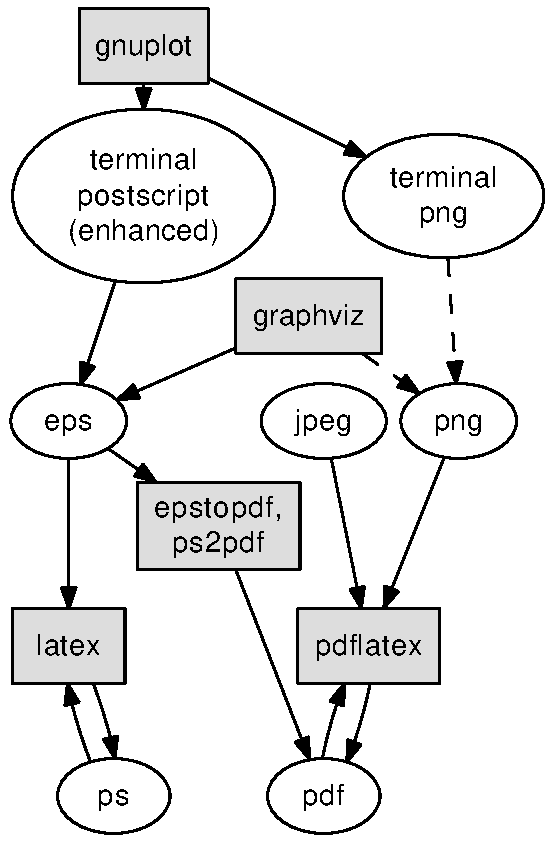
\includegraphics[width=0.4\textwidth]{rys_graf.pdf}
% \end{center}
% \caption{Example diagram from the \emph{graphviz} program, which is a tool that automatically produces diagram layouts~\cite{graphviz}. Remember that wherever possible, we use vector graphics -- avoid embedding bitmaps in the document. In some cases, the use of bitmaps is justified (for quick on-screen previews or for extremely complex graphics containing, for example, hundreds of thousands of objects). The differences in raster and vector graphics are discussed (in Polish) in~\url{https://www.youtube.com/watch?v=_98SDNIpm24}.}
% \label{fig:schemat}
% \end{figure}


% This is a sample text in LaTeX. Read it carefully (the content, its source and the \%comments) and use the \texttt{*.tex} source as a report template -- it shows how to

% \begin{tightlist}
% \item insert a diagram created by graphviz (Fig.~\ref{fig:schemat}),
% \item insert a plot created by gnuplot (Fig.~\ref{fig:3d}) and matplotlib (Fig.~\ref{fig:matplotlib}),
% \item cite bibliography formatted by bibtex~\cite{LS-lectures,Goldberg-2002},
% \item refer to figures, references and parts of the report (for example, Sect.~\ref{sec:typografia}),
% \item as well as to equations: note, usually we do not write the word ``equation'', we just write it like this: In~\eqref{eq:mysterious-equation}, a surprising property of some mathematical transformations is shown.
% \end{tightlist}


% \begin{equation}
% \label{eq:mysterious-equation}
% e^{i \pi} = -1 = \sqrt {-1} \sqrt {-1} = \sqrt {-1 \cdot -1} = \sqrt 1 = 1
% \end{equation}





%\section{The characteristics of a good report}
%
%A good report
%\begin{tightlist}
%\item allows the reader to independently reproduce the experiment (from data to results),
%\item contains no ambiguities,
%\item presents conclusions organized from general to specific,
%\item cites the literature in the text,
%\item does not include oversized listings,
%\item clearly presents the results -- usually using plots,
%\item shows any numerical data with the correct number of significant figures,
%\item is concise and aesthetic.
%\end{tightlist}
%
%\noindent An important rule of thumb when writing any report, thesis or paper is that the accompanying data, figures and plots should always have some sort of associated conclusions -- to avoid overwhelming the reader with tables and graphs that they themselves must interpret, since they could not find the appropriate conclusions in the text. The evaluators of the reports evaluate the conclusions, not the fact that the computations were carried out and proved by the included results. In particular, including just the results and plots without explicitly written conclusions and interpretations is almost worthless from the evaluation point of view -- because it says almost nothing about the author's expertise and reasoning. If such a report, rich in results but deficient in conclusions, were by contrast read by an amateur who wanted to learn something new -- they would hardly learn much. So there must be a balance in the report: the included results must have corresponding conclusions and must be commented on in some way, and the written conclusions must be explicitly supported by the included data (e.g., plots).





%\subsection{Typography}
%\label{sec:typografia}
%
%Remember about the difference between a hyphen\footnote{Read Wikipedia's description of the entry ``Hyphen''.} and a dash -- as well as about citing any source material in the relevant places~\cite{WikiDash}. Cite a specific page, not the general address of the website. Write double quotation marks using ``the method of two marks''. Accordingly, with single quotation marks we distinguish between `opening and closing' ones.
%
%For spell-checking the\ .tex file directly, there is, among others, the \emph{aspell} program. It understands various text encodings and has built-in filters for html and other popular formats. With these filters, it omits keywords specific to a given file format, and only analyzes the actual text. % the backslash before the space cues LaTeX to use a regular space (rather than a widened space). In this case, it is not necessary, but in general, this is how we indicate that any period before a space is not the end of a sentence (such an indication is sometimes needed, because LaTeX by default makes wider spaces after all periods assuming that periods separate sentences -- which is almost always right).
%
%
%
%
%
%
%
%\section{Plots}
%
%\noindent For processing text result files and drawing plots, Python accompanied by the matplotlib library is excellent. They are definitely worth learning! Before you prepare a plot, you can watch tips (in Polish) on creating plots and follow them -- how to make a legible and professional plot:~\url{https://www.youtube.com/watch?v=pfSgcsQ2Mtk}. % the tilde is the non-breaking space -- it sticks adjacent words together.
%
%
%\begin{figure}
%\begin{center}
%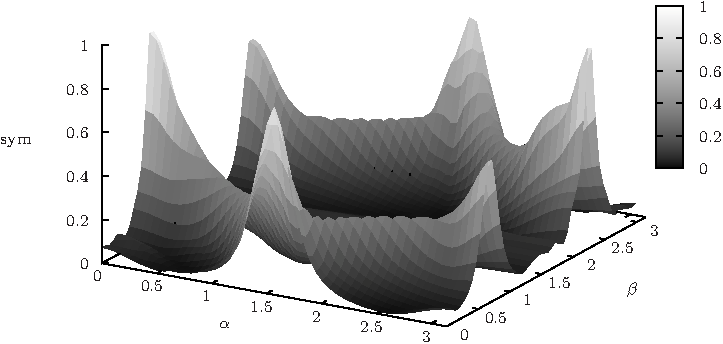
\includegraphics[width=0.9\textwidth]{rys_wykres3d.pdf}
%\end{center}
%\caption{A sample plot, this one produced by the \texttt{gnuplot} program.}
%\label{fig:3d}
%\end{figure}
%
%
%\begin{figure}
%\begin{center}
%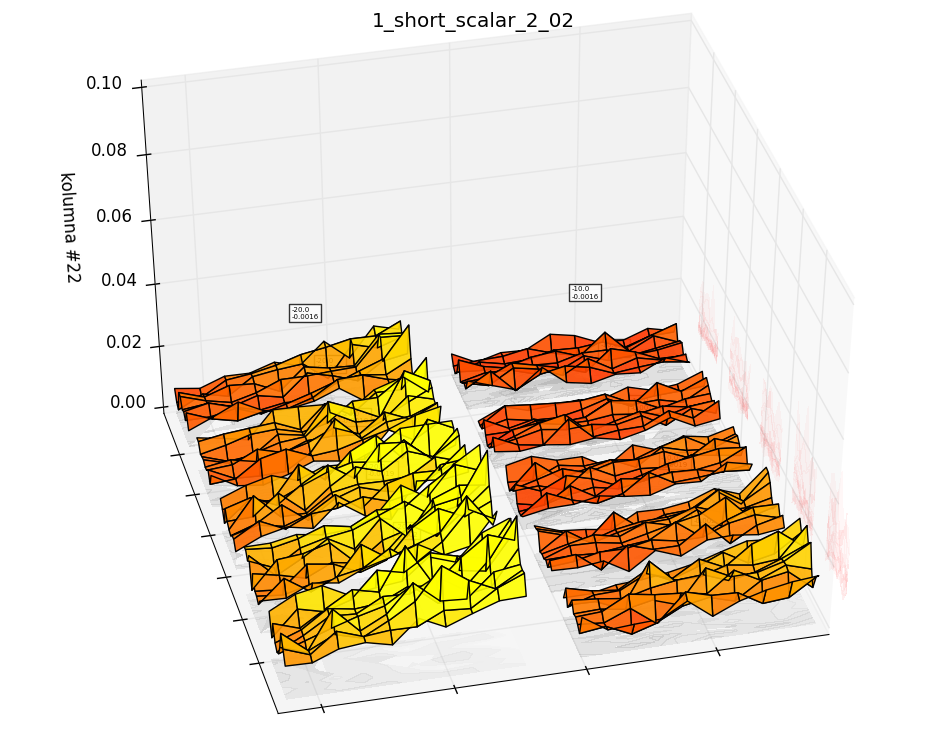
\includegraphics[width=0.48\textwidth]{rys_short_scalar_2_02.png}\hfill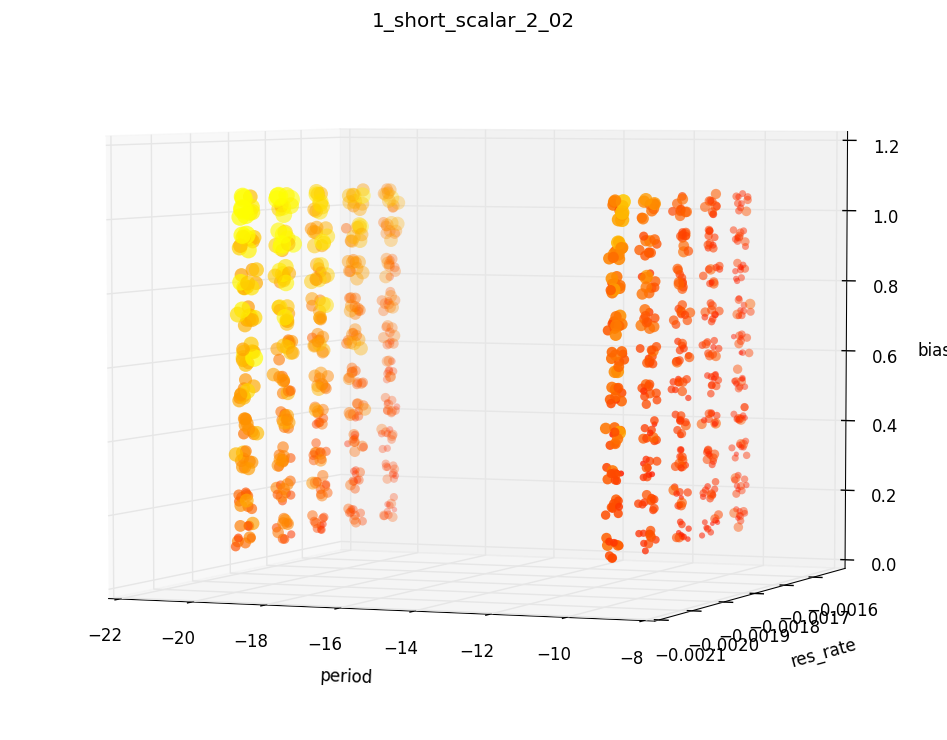
\includegraphics[width=0.48\textwidth]{rys_short_scalar_2_02-kulki.png}
%\end{center}
%\caption{A sample visualization in \texttt{Python}+\texttt{matplotlib}; here, 5D data shown in two ways in 3D. What is wrong with this figure? Bitmaps are used (incorrectly -- should be vector graphics), and the plots here are too small (illegible).}
%\label{fig:matplotlib}
%\end{figure}
%
%\clearpage % let LaTeX put pending figures right here -- this command "releases" the accumulated content, which is useful if you have placed a lot of images, much more than text -- so they do not appear at the end of the document.
%
%
%
%
%
%\section{In closing}
%
%And now something extra. As you have read this entire text source, handle one inconspicuous sentence: \url{http://www.mooncoder.com/latex-challenge.html} %and never again forget what is the difference between hyphens and dashes!


%%%%%%%%%%%%%%%% references %%%%%%%%%%%%%%%%

%\bibliography{biblio}
%\bibliographystyle{plainurl}